% Options for packages loaded elsewhere
% Options for packages loaded elsewhere
\PassOptionsToPackage{unicode}{hyperref}
\PassOptionsToPackage{hyphens}{url}
%
\documentclass[
  ignorenonframetext,
  aspectratio=169,
  handout]{beamer}
\newif\ifbibliography
\usepackage{pgfpages}
\setbeamertemplate{caption}[numbered]
\setbeamertemplate{caption label separator}{: }
\setbeamercolor{caption name}{fg=normal text.fg}
\beamertemplatenavigationsymbolsempty
% remove section numbering
\setbeamertemplate{part page}{
  \centering
  \begin{beamercolorbox}[sep=16pt,center]{part title}
    \usebeamerfont{part title}\insertpart\par
  \end{beamercolorbox}
}
\setbeamertemplate{section page}{
  \centering
  \begin{beamercolorbox}[sep=12pt,center]{section title}
    \usebeamerfont{section title}\insertsection\par
  \end{beamercolorbox}
}
\setbeamertemplate{subsection page}{
  \centering
  \begin{beamercolorbox}[sep=8pt,center]{subsection title}
    \usebeamerfont{subsection title}\insertsubsection\par
  \end{beamercolorbox}
}
% Prevent slide breaks in the middle of a paragraph
\widowpenalties 1 10000
\raggedbottom
\AtBeginPart{
  \frame{\partpage}
}
\AtBeginSection{
  \ifbibliography
  \else
    \frame{\sectionpage}
  \fi
}
\AtBeginSubsection{
  \frame{\subsectionpage}
}
\usepackage{iftex}
\ifPDFTeX
  \usepackage[T1]{fontenc}
  \usepackage[utf8]{inputenc}
  \usepackage{textcomp} % provide euro and other symbols
\else % if luatex or xetex
  \usepackage{unicode-math} % this also loads fontspec
  \defaultfontfeatures{Scale=MatchLowercase}
  \defaultfontfeatures[\rmfamily]{Ligatures=TeX,Scale=1}
\fi
\usepackage{lmodern}

\ifPDFTeX\else
  % xetex/luatex font selection
\fi
% Use upquote if available, for straight quotes in verbatim environments
\IfFileExists{upquote.sty}{\usepackage{upquote}}{}
\IfFileExists{microtype.sty}{% use microtype if available
  \usepackage[]{microtype}
  \UseMicrotypeSet[protrusion]{basicmath} % disable protrusion for tt fonts
}{}
\makeatletter
\@ifundefined{KOMAClassName}{% if non-KOMA class
  \IfFileExists{parskip.sty}{%
    \usepackage{parskip}
  }{% else
    \setlength{\parindent}{0pt}
    \setlength{\parskip}{6pt plus 2pt minus 1pt}}
}{% if KOMA class
  \KOMAoptions{parskip=half}}
\makeatother


\usepackage{longtable,booktabs,array}
\newcounter{none} % for unnumbered tables
\usepackage{calc} % for calculating minipage widths
\usepackage{caption}
% Make caption package work with longtable
\makeatletter
\def\fnum@table{\tablename~\thetable}
\makeatother
\usepackage{graphicx}
\makeatletter
\newsavebox\pandoc@box
\newcommand*\pandocbounded[1]{% scales image to fit in text height/width
  \sbox\pandoc@box{#1}%
  \Gscale@div\@tempa{\textheight}{\dimexpr\ht\pandoc@box+\dp\pandoc@box\relax}%
  \Gscale@div\@tempb{\linewidth}{\wd\pandoc@box}%
  \ifdim\@tempb\p@<\@tempa\p@\let\@tempa\@tempb\fi% select the smaller of both
  \ifdim\@tempa\p@<\p@\scalebox{\@tempa}{\usebox\pandoc@box}%
  \else\usebox{\pandoc@box}%
  \fi%
}
% Set default figure placement to htbp
\def\fps@figure{htbp}
\makeatother





\setlength{\emergencystretch}{3em} % prevent overfull lines

\providecommand{\tightlist}{%
  \setlength{\itemsep}{0pt}\setlength{\parskip}{0pt}}



 


\makeatletter
\@ifpackageloaded{caption}{}{\usepackage{caption}}
\AtBeginDocument{%
\ifdefined\contentsname
  \renewcommand*\contentsname{Table of contents}
\else
  \newcommand\contentsname{Table of contents}
\fi
\ifdefined\listfigurename
  \renewcommand*\listfigurename{List of Figures}
\else
  \newcommand\listfigurename{List of Figures}
\fi
\ifdefined\listtablename
  \renewcommand*\listtablename{List of Tables}
\else
  \newcommand\listtablename{List of Tables}
\fi
\ifdefined\figurename
  \renewcommand*\figurename{Figure}
\else
  \newcommand\figurename{Figure}
\fi
\ifdefined\tablename
  \renewcommand*\tablename{Table}
\else
  \newcommand\tablename{Table}
\fi
}
\@ifpackageloaded{float}{}{\usepackage{float}}
\floatstyle{ruled}
\@ifundefined{c@chapter}{\newfloat{codelisting}{h}{lop}}{\newfloat{codelisting}{h}{lop}[chapter]}
\floatname{codelisting}{Listing}
\newcommand*\listoflistings{\listof{codelisting}{List of Listings}}
\makeatother
\makeatletter
\makeatother
\makeatletter
\@ifpackageloaded{caption}{}{\usepackage{caption}}
\@ifpackageloaded{subcaption}{}{\usepackage{subcaption}}
\makeatother

\usepackage{bookmark}
\IfFileExists{xurl.sty}{\usepackage{xurl}}{} % add URL line breaks if available
\urlstyle{same}
\hypersetup{
  pdftitle={The Wave Equation},
  pdfauthor={Davit Potoyan},
  hidelinks,
  pdfcreator={LaTeX via pandoc}}


\title{\texorpdfstring{The Wave Equation}{The Wave Equation}}
\subtitle{\texorpdfstring{Chem 3240 · Lecture
2.2}{Chem 3240 · Lecture 2.2}}
\author{Davit Potoyan}
\date{}

\begin{document}
\frame{\titlepage}


\begin{frame}
\begin{block}{The Classical Wave Equation}
\protect\phantomsection\label{the-classical-wave-equation}
\begin{columns}[T]
\begin{column}{0.5\linewidth}
\includegraphics[width=0.9\linewidth,height=\textheight,keepaspectratio]{../../ch02/images/1D-Wave.gif}
\end{column}

\begin{column}{0.5\linewidth}
\begin{itemize}
\tightlist
\item
  A second-order \textbf{PDE} for the displacement \(u(x,t)\)
\end{itemize}

\[\frac{\partial^2 u(x,t)}{\partial x^2} = \frac{1}{v^2}\frac{\partial^2 u(x,t)}{\partial t^2}\]

\begin{itemize}
\tightlist
\item
  Governs evolution in \textbf{space and time}
\item
  Given initial conditions, predicts any complicated wave
\end{itemize}
\end{column}
\end{columns}
\end{block}

\begin{block}{Why a Guitar String?}
\protect\phantomsection\label{why-a-guitar-string}
\begin{columns}[T]
\begin{column}{0.5\linewidth}
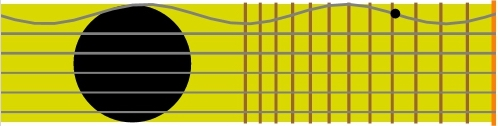
\includegraphics[width=0.9\linewidth,height=\textheight,keepaspectratio]{../../ch02/images/lec5_guitar.jpg}
\end{column}

\begin{column}{0.5\linewidth}
\begin{itemize}
\tightlist
\item
  A plucked string is the classic \textbf{1D wave} system
\item
  Specify initial conditions, predict evolution over space and time
\item
  \textbf{Linear} PDE: any combination of solutions is a solution
\end{itemize}
\end{column}
\end{columns}
\end{block}

\begin{block}{The Big Picture: Three Ingredients}
\protect\phantomsection\label{the-big-picture-three-ingredients}
\begin{itemize}
\tightlist
\item
  \textbf{1. Boundary conditions} (string fixed at both ends):
\end{itemize}

\[u(0, t) = 0 \quad \text{and} \quad u(L, t) = 0\]

\begin{itemize}
\tightlist
\item
  \textbf{2. Separation of variables} (assume \(x\), \(t\) vary
  independently):
\end{itemize}

\[u(x, t) = X(x) \cdot T(t)\]

\begin{itemize}
\tightlist
\item
  \textbf{3. Superposition} (linearity lets us sum solutions):
\end{itemize}

\[u = c_1 u_1+c_2u_2\]
\end{block}

\begin{block}{Step 1: Separate the Variables}
\protect\phantomsection\label{step-1-separate-the-variables}
\begin{itemize}
\tightlist
\item
  Substitute \(u(x,t) = X(x)T(t)\) into the wave equation
\item
  Divide through: each side depends on \textbf{one variable only}, so
  both equal a constant \(K\)
\end{itemize}

\[\frac{1}{T(t)v^2}\frac{\partial^2 T(t)}{\partial t^2} = \frac{1}{X(x)}\frac{\partial^2 X(x)}{\partial x^2} = K\]

\begin{itemize}
\tightlist
\item
  One \textbf{PDE} becomes two \textbf{ODEs}:
\end{itemize}

\[\frac{\partial^2 T(t)}{\partial t^2} - K T(t) v^2 = 0 \qquad \frac{\partial^2 X(x)}{\partial x^2} - K X(x) = 0\]
\end{block}

\begin{block}{Step 2: The Sign of K Decides}
\protect\phantomsection\label{step-2-the-sign-of-k-decides}
\begin{itemize}
\tightlist
\item
  \textbf{Recipe for linear, homogeneous ODEs:} plug in
  \(y \to e^{kx}\), solve the algebraic equation for \(k\)
\item
  \textbf{\(K > 0\):} real exponentials, boundary conditions force
  \(X(x) = 0\) (no music!)
\item
  \textbf{\(K < 0\)} (set \(K = -\beta^2\)): oscillatory solution
\end{itemize}

\[X(x) = A \cos(\beta x) + B \sin(\beta x)\]

\begin{itemize}
\tightlist
\item
  Boundary conditions: \(A = 0\), and \(\sin(\beta L) = 0\) for a
  non-trivial solution
\end{itemize}
\end{block}

\begin{block}{Normal Modes Emerge}
\protect\phantomsection\label{normal-modes-emerge}
\begin{columns}[T]
\begin{column}{0.5\linewidth}
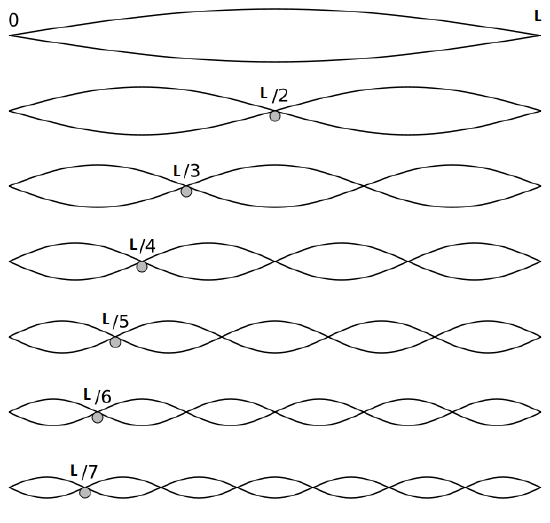
\includegraphics[width=0.9\linewidth,height=\textheight,keepaspectratio]{../../ch02/images/modes-x.png}
\end{column}

\begin{column}{0.5\linewidth}
\begin{itemize}
\tightlist
\item
  \(\sin(\beta L) = 0\) quantizes \(\beta\):
\end{itemize}

\[\beta = \frac{n \pi}{L}, \quad n = 1, 2, 3, \ldots\]

\begin{itemize}
\tightlist
\item
  Infinite set of \textbf{normal modes}:
\end{itemize}

\[X(x) = B \sin \left(\frac{n \pi}{L} x \right)\]
\end{column}
\end{columns}
\end{block}

\begin{block}{The Temporal Part}
\protect\phantomsection\label{the-temporal-part}
\begin{itemize}
\tightlist
\item
  Time has \textbf{no boundary conditions}: it marches forward freely
\item
  Solution is oscillatory with mode frequency
  \(\omega_n = \beta v = \frac{n \pi v}{L}\)
\end{itemize}

\[T(t) = D_n \cos(\omega_n t) + E_n \sin(\omega_n t) = A_n \cos (\omega_n t + \phi_n)\]

\begin{itemize}
\tightlist
\item
  Constants \(A_n\) and \(\phi_n\) are fixed by \textbf{initial
  conditions} (how the string is plucked)
\end{itemize}
\end{block}

\begin{block}{Step 3: The Full Solution}
\protect\phantomsection\label{step-3-the-full-solution}
\begin{itemize}
\tightlist
\item
  Combine spatial and temporal parts, sum over all modes:
\end{itemize}

\[u(x, t) = \sum_n A_n \sin \left(\frac{n \pi}{L} x \right) \cdot \cos (\omega_n t + \phi_n)\]

\begin{itemize}
\tightlist
\item
  \textbf{Nodes} (points fixed at zero) grow with \(n\):

  \begin{itemize}
  \tightlist
  \item
    \(n=1\): \textbf{0 nodes}, fundamental (first harmonic)
  \item
    \(n=2\): 1 node, second harmonic
  \item
    \(n=3\): 2 nodes, third harmonic
  \end{itemize}
\end{itemize}
\end{block}

\begin{block}{Extending to 2D Membranes}
\protect\phantomsection\label{extending-to-2d-membranes}
\begin{columns}[T]
\begin{column}{0.5\linewidth}
\includegraphics[width=0.9\linewidth,height=\textheight,keepaspectratio]{../../ch02/images/2dmemvib.gif}
\end{column}

\begin{column}{0.5\linewidth}
\begin{itemize}
\tightlist
\item
  Separate \textbf{three} functions: \(u(x, y, t) = X(x) Y(y) T(t)\)
\item
  2D mode is a product of 1D modes, indexed by \(n\) and \(m\)
\end{itemize}

\[\omega_{nm} = v\pi \left(\frac{n^2}{a^2} + \frac{m^2}{b^2}\right)^{1/2}\]
\end{column}
\end{columns}
\end{block}

\begin{block}{The Sound of Music}
\protect\phantomsection\label{the-sound-of-music}
\begin{columns}[T]
\begin{column}{0.5\linewidth}
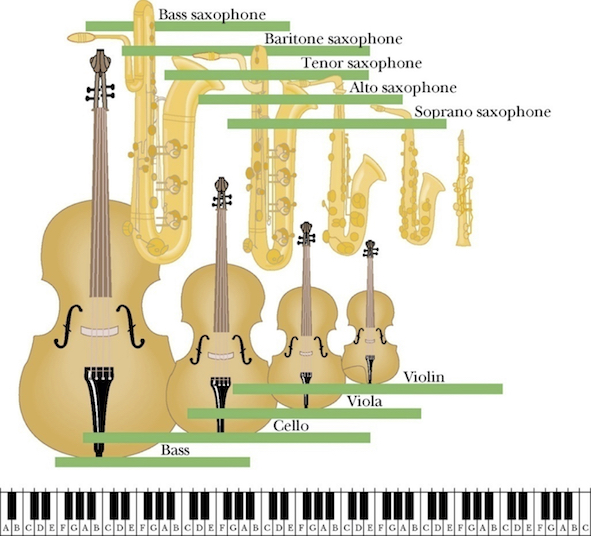
\includegraphics[width=0.9\linewidth,height=\textheight,keepaspectratio]{../../ch02/images/lec4_music.jpg}
\end{column}

\begin{column}{0.5\linewidth}
\begin{itemize}
\tightlist
\item
  Musical sound is a \textbf{superposition of normal modes} (harmonics,
  overtones)
\item
  Instrument \textbf{size} sets the frequency range: small = high, large
  = low
\end{itemize}
\end{column}
\end{columns}
\end{block}
\end{frame}

\begin{frame}{Takeaway}
\protect\phantomsection\label{takeaway}
\begin{quote}
Separation of variables plus boundary conditions turns the wave equation
into quantized \textbf{normal modes}, and any vibration is a
superposition of them.
\end{quote}
\end{frame}




\end{document}
